\appendix

\section{Implementation Details}
\label{sec:appendix-implementation}

The pipeline is Python, one module per stage of \S\ref{sec:method}: rendering/extraction via Playwright (\code{dom\_extraction.py}); tiling and pruning over Pillow crops (\code{tiling.py}); graph construction with \code{networkx} (\code{graph\_builder.py}); the reader VLM via Ollama (\texttt{qwen3-vl}, default, no GPU needed) or Hugging Face \code{transformers} (\code{Qwen2-VL-7B-Instruct}) for LoRA fine-tuning, every call cached to disk by a hash of (image, prompt, decoding-config) since decoding is greedy, so a retried page never re-pays a call already made (\code{vlm\_client.py}); synthetic QA generation (\code{qa\_generation.py}); hard-negative mining via \code{scikit-learn} TF-IDF with a dependency-free fallback (\code{hard\_negative\_mining.py}); and contrastive LoRA fine-tuning with \code{peft}/\code{torch}, target modules discovered by introspecting the loaded model rather than hard-coded (\code{lora\_finetune.py}).

\paragraph{Oversized-page splitting, composition, and concurrency.} \code{sectioning.py} implements the \code{h1}/\code{h2} split as a pure function over already-extracted elements, unit-testable without Playwright. \code{corpus\_builder.py} separates network-bound fetch from a synchronous core that tiles, decides whether to split, and composes per-section graphs, exposing an \code{entry\_page} on every graph; multi-page (\code{links\_to}) and multi-section (\code{continues}) composition share the same node-namespacing machinery. QA generation issues per-tile VLM calls concurrently within a page (a thread pool sized to Ollama's default parallelism); the controller does the same on the query path, since which nodes open depends only on relevance scores computed upfront, never on a VLM response.

\paragraph{Batch construction and resolution ablation.} \code{scripts/build\_dataset.py} drives the pipeline over a page list with retrying fetches; its unit of work is a \emph{page unit} (a page, or one split section), checkpointed independently to \code{contrastive\_examples.jsonl} -- a failure partway through an oversized page costs only the section in flight, motivated by an early run that lost hours of work when the whole page was the retry unit. \code{image\_compression.py} mirrors tile images at a reduced scale under a separate root with identical filenames and relative paths, so switching a training run between resolutions (\S\ref{sec:contrastive}) is a single \code{-{}-images-root} flag.

\paragraph{Tiling ablation and multi-hop data.} \code{scripts/grid\_baseline.py} reimplements the blind grid as a module independent of \code{tiling.py}; \code{scripts/dom\_vs\_grid\_experiment.py} re-renders each page, builds both tilings, and ranks existing questions against both by TF-IDF (\S\ref{sec:experiments}). Its oversized-page check uses a threshold local to the ablation (25$\times$ \code{MAX\_TILE\_HEIGHT}, vs.\ 10$\times$ for \code{build\_dataset.py}'s own split decision) since, unlike corpus construction, this ablation never calls the VLM and so does not carry the same runaway-generation-time risk that motivates the tighter default; \code{scripts/pin\_wikipedia\_snapshot.py} freezes each page's Wikipedia revision beforehand so the ablation is reproducible across runs despite live articles growing over time. \code{src/multihop\_qa.py} builds cross-page examples from HotpotQA~\citep{hotpotqa2018} records streamed via the \code{datasets} library; \code{scripts/build\_multihop\_dataset.py} reports unreachable-article vs.\ unmatched-sentence drops separately. Positive-tile attribution uses stopword-filtered token overlap rather than exact substring matching, since the latter rarely survives a decade of article edits since HotpotQA's 2017 source dump.

\paragraph{Demonstration and tests.} A notebook runs every stage end-to-end with interactive \code{pyvis} graph visualizations. Dependency-light unit tests cover the geometric pipeline, graph construction and splitting, hard-negative mining (lexical and VLM-judge, stub client), the VLM cache and call concurrency, and resolution compression, all on synthetic fixtures needing no network, VLM, or GPU. Playwright-backed tests check the text-flow bounding-box measurement (floated-sidebar fixture) and the full geometric pipeline end-to-end (DOM extraction through XML export) against a bundled local HTML fixture.

\section{Hyperparameters}
\label{sec:appendix-hyperparams}

Every hyperparameter referenced in \S\ref{sec:tiling}--\S\ref{sec:contrastive}, in one place.

\begin{table}[h]
\centering
\small
\begin{tabular}{@{}lr@{}}
\toprule
Parameter & Value \\
\midrule
Viewport / max tile width & 2048\,px \\
Max tile height (patching) & 2048\,px \\
VLM \code{max\_pixels} (unmodified default) & $28{\times}28{\times}1280 \approx 1.00$M px \\
Min tile height (merging) & 80\,px \\
Row-grouping tolerance & 20\,px \\
Nesting tolerance & 1\,px \\
Overlap-grouping threshold & 15\% of smaller area \\
Link-bearing tiles kept ($k$) & 3 \\
Oversize-split threshold & $10\times$ max tile height \\
Mined hard negatives ($n$) & 2 \\
Semantic-neighbor threshold & 0.2 cosine \\
Semantic neighbors / tile (max) & 3 \\
Downscale factor (ablation) & 0.5 \\
LoRA $r$ / $\alpha$ / dropout & 16 / 32 / 0.05 \\
InfoNCE temperature $\tau$ & 0.05 \\
\bottomrule
\end{tabular}
\caption{All pipeline hyperparameters (\S\ref{sec:tiling}--\S\ref{sec:contrastive}). Each is a single documented, centralized value, not swept; see \S\ref{sec:limitations}.}
\label{tab:appendix-hyperparams}
\end{table}

\section{Compute budget for contrastive fine-tuning}
\label{sec:appendix-gpu}

Training (ablation (b)) ran on a rented 80\,GB A100/H100-class card, batch size 4, $n{=}2$ hard negatives, 3 epochs over the 1{,}339 examples of Table~\ref{tab:dataset-stats}. The batched embedding path (\code{lora\_finetune.py}, default) first hit \texttt{torch.OutOfMemoryError} on a routine \code{dropout} call with 79.16 of 79.25\,GiB already in use -- genuine peak usage, not fragmentation, since our largest tiles ($2048\times2048$\,px) push a large vision-token count through the batch jointly. \code{-{}-gradient-checkpointing} (recomputing activations on the backward pass, $\sim$20--30\% slower) resolved it and should be treated as the default starting point at this tile resolution on an 80\,GB card, not a fallback for smaller ones only.

\section{Tiling ablation: cost detail}
\label{sec:appendix-tiling-cost}

Per-tile breakdown behind the pixel-budget figure reported in \S\ref{sec:experiments} (ablation (a)).

\begin{table}[h]
\centering
\small
\begin{tabular}{@{}lrrr@{}}
\toprule
 & Tiles/page & Px/tile & Total px/page \\
\midrule
DOM  & 24.0 & 159{,}558 & 3{,}829{,}395 \\
Grid & 4.9  & 2{,}065{,}749 & 10{,}213{,}983 \\
\bottomrule
\end{tabular}
\caption{Tiling cost, same 18 pages as Table~\ref{tab:tiling-ablation}. DOM-guided tiling produces more, smaller tiles, yet a smaller \emph{total} pixel budget per page (2.7$\times$ less) -- a direct consequence of the text-flow bounding-box measurement of \S\ref{sec:tiling}, which crops text tiles to the width their content actually occupies instead of the full page width every grid band uses regardless of content.}
\label{tab:appendix-tiling-cost}
\end{table}

\paragraph{From pixels to tokens.} The 2.7$\times$ figure above is a pixel ratio, not a token ratio, and image tokens track pixel area only below \texttt{Qwen2-VL}'s preprocessor cap. \code{AutoProcessor.from\_pretrained} is called with no \code{max\_pixels} override (\code{vlm\_client.py}, \code{lora\_finetune.py}), so the shipped default applies: $28\times28\times1280\approx1.00$M px per tile (Appendix~\ref{sec:appendix-hyperparams}), above which the processor downscales a tile before encoding rather than tokenizing its raw area. Our DOM tiles (159{,}558\,px average) sit comfortably under this cap throughout, so their token cost tracks their pixel area; our grid bands (2{,}065{,}749\,px average) sit roughly $2\times$ over it, so each is downscaled to the cap and contributes a near-constant $\sim$1{,}280 tokens regardless of its raw size, rather than the $\sim$2{,}635 tokens its uncapped area would imply. Propagating both tile counts through this cap gives an estimated mean of $\sim$4{,}910 tokens/page for DOM tiling against $\sim$6{,}330 for the grid, across the same 18 pages -- roughly $1.3\times$, not $2.7\times$. The direction of the result is unaffected; the pixel-budget figure above should be read as a pixel claim only, since we did not instrument the processor to confirm these token counts directly.

\section{Additional figures}
\label{sec:appendix-figures}

\begin{figure}[h]
\centering
\begin{tikzpicture}[
  scale=0.8, transform shape,
  node distance=1.1cm and 1.6cm,
  st/.style={draw, rounded corners, minimum width=1.9cm, minimum height=0.65cm, align=center, font=\small},
  arr/.style={-{Stealth[length=2mm]}, thick}
]
\node[st] (inactive) {\state{inactive}};
\node[st, right=of inactive] (active) {\state{active}};
\node[st, above right=0.5cm and 1.5cm of active] (opened) {\state{opened}};
\node[st, below right=0.5cm and 1.5cm of active] (pruned) {\state{pruned}};
\draw[arr] (inactive) -- node[above, font=\scriptsize]{activate} (active);
\draw[arr] (active) -- node[above, sloped, font=\scriptsize]{open (budget --1)} (opened);
\draw[arr] (active) -- node[below, sloped, font=\scriptsize]{prune (free)} (pruned);
\end{tikzpicture}
\caption{The controller's state machine (\S\ref{sec:controller}). Opening a node consumes budget and may activate inactive neighbors (\code{reading\_order}, or across a document boundary via \code{links\_to}/\code{continues}); pruning is free, applied to any node still \state{active} once budget is exhausted.}
\label{fig:states}
\end{figure}

\begin{figure*}[h]
\centering
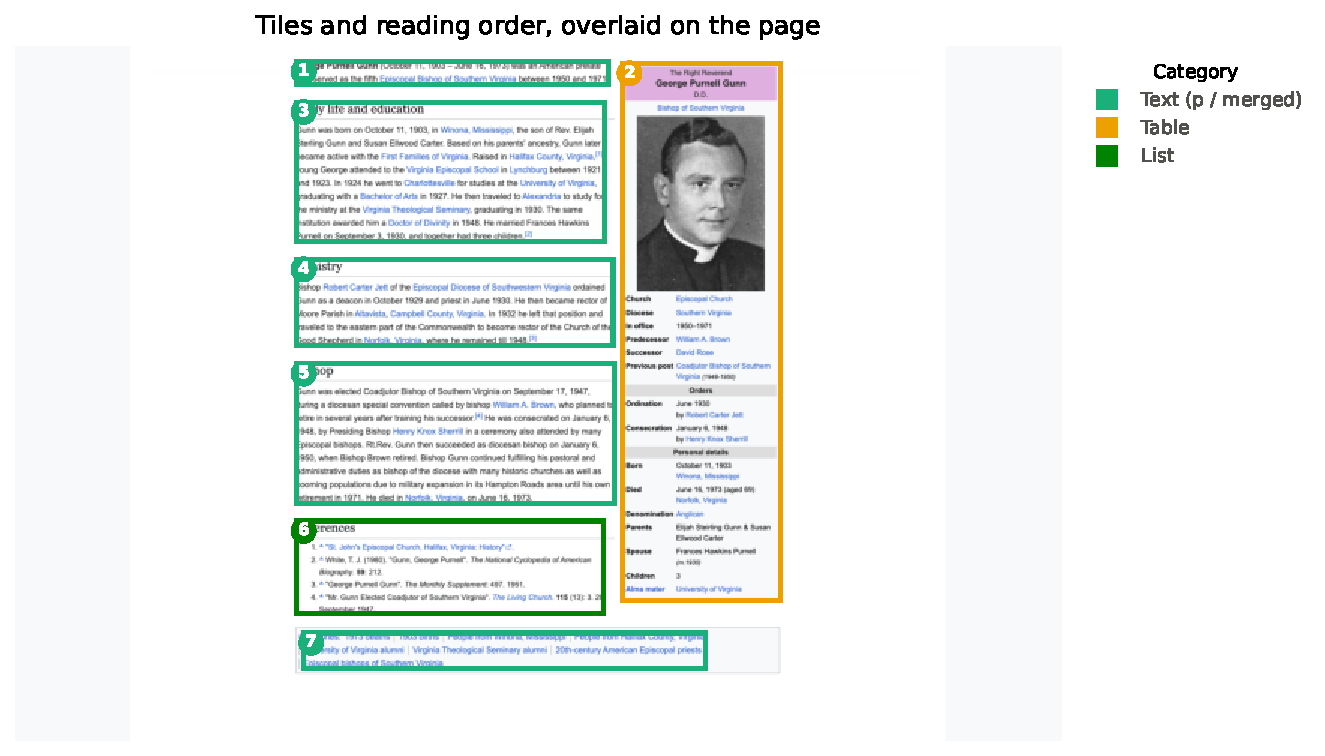
\includegraphics[width=0.62\textwidth]{figures/tiling_overlay.pdf}
\caption{DOM-guided tiles (colored by content category, numbered in reading order) overlaid on the rendered page for \texttt{en.wikipedia.org/wiki/George\_P.\_Gunn}. Tile boundaries follow the DOM's own element boundaries: the infobox table (tile 2) is never split mid-row and stays disjoint from the body text and reference list that visually share its column range (tiles 1, 3--6), each section heading is paired with its first content block -- a paragraph for tiles 3--5, the reference list itself for tile 6 -- rather than emitted alone, and the trailing category footer (tile 7) is merged into its own tile rather than left as a flood of near-empty fragments.}
\label{fig:tiling-overlay}
\end{figure*}

\begin{figure*}[h]
\centering
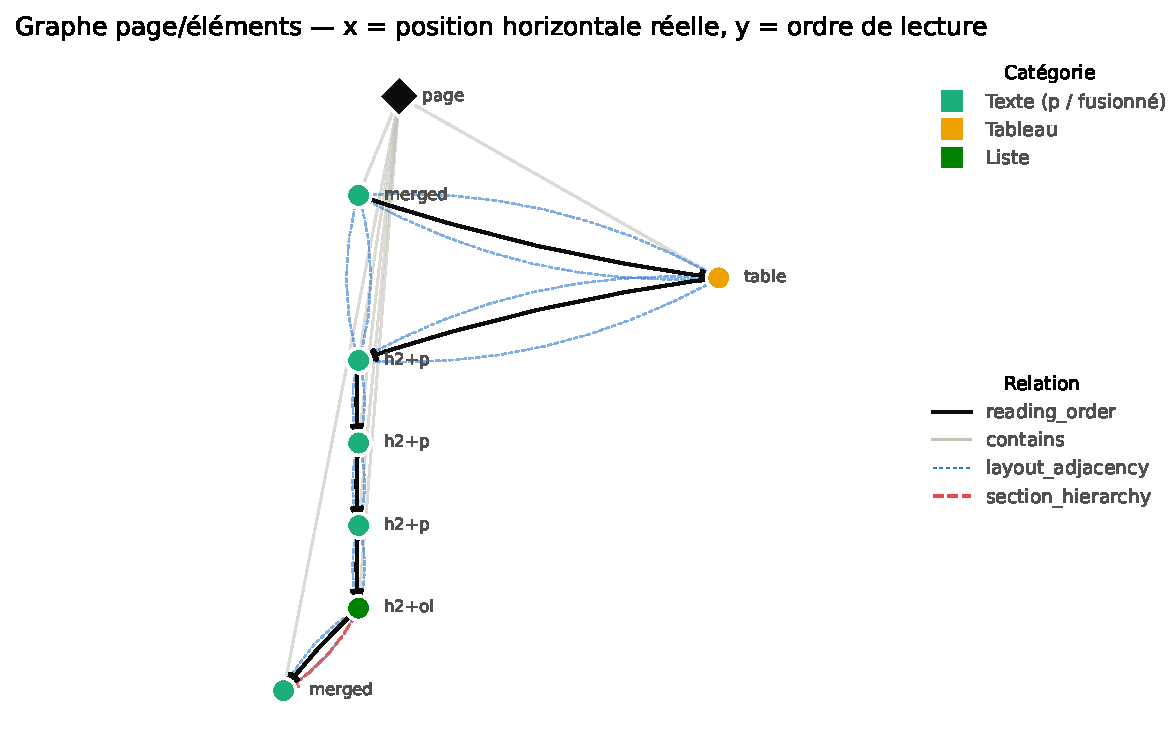
\includegraphics[width=0.55\textwidth]{figures/page_graph.pdf}
\caption{Page/element graph for the same page as Figure~\ref{fig:tiling-overlay}, laid out by real horizontal position ($x$) and reading-order rank ($y$). \code{reading\_order} (solid black) and \code{contains} (light gray) are the two relations MAGE-RAG also has; \code{layout\_adjacency} (dotted blue) and \code{section\_hierarchy} (dashed red) are the two we add. Most headings here are paired with their content into one tile (\S\ref{sec:tiling}), so \code{section\_hierarchy} shows only where trailing non-heading content (the category footer) attaches to the last open section, rather than between the (sibling, not nested) section headings themselves.}
\label{fig:page-graph}
\end{figure*}

\begin{figure*}[h]
\centering
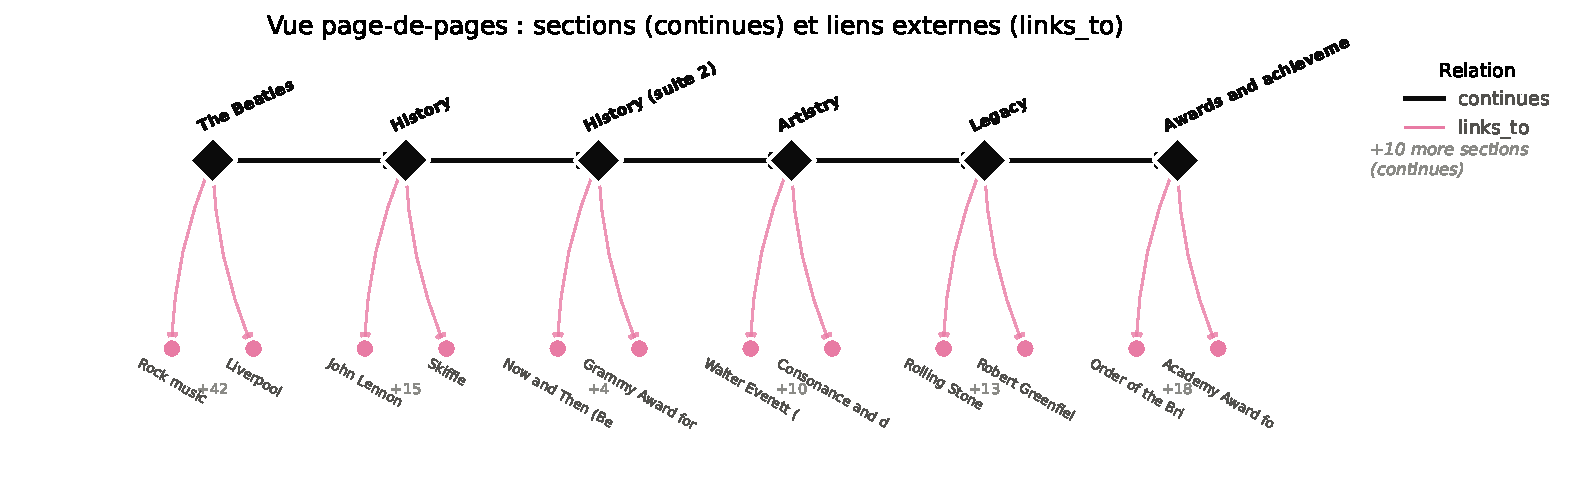
\includegraphics[width=0.85\textwidth]{figures/section_split_overview.pdf}
\caption{Page-level view of the graph for \texttt{en.wikipedia.org/wiki/The\_Beatles} (278 DOM elements, split into 16 sections at \code{h1}/\code{h2} boundaries -- only the first 6 are shown for legibility). Each diamond is a \code{page} node, one per section; \code{continues} edges (black) chain them in document order; \code{links\_to} edges (pink) reach external pages, collapsed here from their true element-level source (\S\ref{sec:graph}) to stay at page granularity. The leftmost node is the entry point.}
\label{fig:section-split}
\end{figure*}

\begin{figure}[h]
\centering
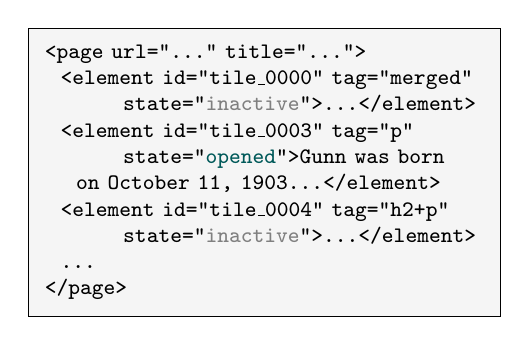
\begin{tikzpicture}[font=\footnotesize]
\node[draw, rectangle, fill=gray!8, align=left, text width=0.46\textwidth, inner sep=6pt] (xml) {
\ttfamily
<page url="..." title="..."> \\
\ \ <element id="tile\_0000" tag="merged"\\
\ \ \ \ \ \ \ \ \ \ state="\textcolor{gray}{inactive}">...</element> \\
\ \ <element id="tile\_0003" tag="p"\\
\ \ \ \ \ \ \ \ \ \ state="\textcolor{teal!70!black}{opened}">Gunn was born\\
\ \ \ \ on October 11, 1903...</element> \\
\ \ <element id="tile\_0004" tag="h2+p"\\
\ \ \ \ \ \ \ \ \ \ state="\textcolor{gray}{inactive}">...</element> \\
\ \ ...\\
</page>
};
\end{tikzpicture}
\caption{Excerpt of the XML rendering of a page graph after the evidence controller has run on the query ``When and where was George Purnell Gunn born?''. Only the paragraph tile carrying the birth date/place has been opened; the rest remains inactive or pruned.}
\label{fig:xml}
\end{figure}
